\chapter{راهنمای استفاده از کلاس}
\thispagestyle{empty}
\section{مقدمه}
حروف‌چینی پروژه کارشناسی، پایان‌نامه یا رساله یکی از موارد پرکاربرد استفاده از زی‌پرشین است. از طرفی، یک پروژه، پایان‌نامه یا رساله،  احتیاج به تنظیمات زیادی از نظر صفحه‌آرایی  دارد که ممکن است برای
یک کاربر مبتدی، مشکل باشد. به همین خاطر، برای راحتی کار کاربر، کلاس حاضر با نام 
 \LRE{\verb!tabriz-thesis!}
 برای حروف‌چینی پروژه‌ها، پایان‌نامه‌ها و رساله‌های دانشگاه تبریز با استفاده از نرم‌افزار زی‌پرشین،  آماده شده است. این فایل به 
گونه‌ای طراحی شده است که کلیه خواسته‌های مورد نیاز  مدیریت تحصیلات تکمیلی دانشگاه تبریز را برآورده می‌کند و نیز، حروف‌چینی بسیاری
از قسمت‌های آن، به طور خودکار انجام می‌شود.

کلیه فایل‌های لازم برای حروف‌چینی با کلاس گفته شده، داخل پوشه‌ای به نام
 \LRE{\verb!tabriz-thesis!}
  قرار داده شده است. توجه داشته باشید که برای استفاده از این کلاس باید فونت‌های
\LRE{\verb!XB Niloofar!}،
 \verb!Yas!
 و
  \verb!IranNastaliq!
    روی سیستم شما نصب شده باشد.
\section{این همه فایل؟!}\label{sec2}
از آنجایی که یک پایان‌نامه یا رساله، یک نوشته بلند محسوب می‌شود، لذا اگر همه تنظیمات و مطالب پایان‌نامه را داخل یک فایل قرار بدهیم، باعث شلوغی
و سردرگمی می‌شود. به همین خاطر، قسمت‌های مختلف پایان‌نامه یا رساله  داخل فایل‌های جداگانه قرار گرفته است. مثلاً تنظیمات پایه‌ای کلاس، داخل فایل
\LRE{\verb!tabriz-thesis.cls!}، 
تنظیمات قابل تغییر توسط کاربر، داخل 
\verb!commands.tex!،
قسمت مشخصات فارسی پایان‌نامه، داخل 
\LRE{\verb!fa-title.tex!}،
مطالب فصل اول، داخل 
\verb!chapter1!
و ... قرار داده شده است. نکته مهمی که در اینجا وجود دارد این است که از بین این  فایل‌ها، فقط فایل 
\LRE{\verb!tabriz-thesis.tex!}
قابل اجرا است. یعنی بعد از تغییر فایل‌های دیگر، برای دیدن نتیجه تغییرات، باید این فایل را اجرا کرد. بقیه فایل‌ها به این فایل، کمک می‌کنند تا بتوانیم خروجی کار را ببینیم. اگر به فایل 
\LRE{\verb!tabriz-thesis.tex!}
دقت کنید، متوجه می‌شوید که قسمت‌های مختلف پایان‌نامه، توسط دستورهایی مانند 
\verb!input!
و
\verb!include!
به فایل اصلی، یعنی 
\LRE{\verb!tabriz-thesis.tex!}
معرفی شده‌اند. بنابراین، فایلی که همیشه با آن سروکار داریم، فایل 
\LRE{\verb!tabriz-thesis.tex!}
است.
در این فایل، فرض شده است که پایان‌نامه یا رساله، از ۳ فصل و یک پیوست، تشکیل شده است. با این حال، اگر
  پایان‌نامه یا رساله، بیشتر از ۳ فصل و یک پیوست است، باید خودتان فصل‌های بیشتر را به این فایل، اضافه کنید. این کار، بسیار ساده است. فرض کنید بخواهید یک فصل دیگر هم به پایان‌نامه، اضافه کنید. برای این کار، کافی است یک فایل با نام 
\verb!chapter4!
و با پسوند 
\verb!.tex!
بسازید و آن را داخل پوشه 
\LRE{\verb!tabriz-thesis!}
قرار دهید و سپس این فایل را با دستور 
\verb!\include{chapter4}!
داخل فایل
\LRE{\verb!tabriz-thesis.tex!}
و بعد از دستور
\verb!\chapter{اندازه‌ها و ارزیابی‌ها}
\thispagestyle{empty}
\section{اندازه‌ها و تابعی‌های خطی مثبت روی $\mathrm{C(X)}$}
فرض کنید $X$ یک فضای توپولوژیکی روی ...
\section{تابعی‌های خطی}
در این بخش ...!
 قرار دهید.
\section{از کجا شروع کنم؟}
قبل از هر چیز، بدیهی است که باید یک توزیع تِک مناسب مانند 
\verb!Live TeX!
و یک ویرایش‌گر تِک مانند
\verb!Texmaker!
را روی سیستم خود نصب کنید.  نسخه بهینه شده \verb!Texmaker!  را می‌توانید  از سایت 
 \href{http://www.parsilatex.com}{پارسی‌لاتک}%
\LTRfootnote{\url{http://www.parsilatex.com}}
 و \verb!Live TeX!  را هم می‌توانید از 
 \href{http://www.tug.org/texlive}{سایت رسمی آن}%
\LTRfootnote{\url{http://www.tug.org/texlive}}
 دانلود کنید.
 
در مرحله بعد، سعی کنید که  یک پشتیبان از پوشه 
\LRE{\verb!tabriz-thesis!}
 بگیرید و آن را در یک جایی از هارددیسک سیستم خود ذخیره کنید تا در صورت خراب کردن فایل‌هایی که در حال حاضر، با آن‌ها کار می‌کنید، همه چیز را از 
 دست ندهید.
 
 حال اگر نوشتن \پ اولین تجربه شما از کار با لاتک است، توصیه می‌شود که یک‌بار به طور سرسری، کتاب «%
\href{http://www.tug.ctan.org/tex-archive/info/lshort/persian/lshort.pdf}{مقدمه‌ای نه چندان کوتاه بر
\lr{\LaTeXe}}\LTRfootnote{\url{http://www.tug.ctan.org/tex-archive/info/lshort/persian/lshort.pdf}}»
   ترجمه دکتر مهدی امیدعلی، عضو هیات علمی دانشگاه شاهد را مطالعه کنید. این کتاب، کتاب بسیار کاملی است که خیلی از نیازهای شما در ارتباط با حروف‌چینی را برطرف می‌کند.
 
 
بعد از موارد گفته شده، فایل 
\LRE{\verb!tabriz-thesis.tex!}
و
\LRE{\verb!fa-title!}
را باز کنید و مشخصات پایان‌نامه خود مثل نام، نام خانوادگی، عنوان پایان‌نامه و ... را جایگزین مشخصات موجود در فایل
\LRE{\verb!fa-title!}
 کنید. دقت داشته باشید که نیازی نیست 
نگران چینش این مشخصات در فایل پی‌دی‌اف خروجی باشید. فایل 
\LRE{\verb!tabriz-thesis.cls!}
همه این کارها را به طور خودکار برای شما انجام می‌دهد. در ضمن، موقع تغییر دادن دستورهای داخل فایل
\LRE{\verb!fa-title!}
 کاملاً دقت کنید. این دستورها، خیلی حساس هستند و ممکن است با یک تغییر کوچک، موقع اجرا، خطا بگیرید. برای دیدن خروجی کار، فایل 
\LRE{\verb!fa-title!}
 را 
\verb!Save!، 
(نه 
\verb!As Save!)
کنید و بعد به فایل 
\LRE{\verb!tabriz-thesis.tex!}
برگشته و آن را اجرا کنید. حال اگر می‌خواهید مشخصات انگلیسی \پ را هم عوض کنید، فایل 
\LRE{\verb!en-title!}
را باز کنید و مشخصات داخل آن را تغییر دهید.%
\RTLfootnote{
برای نوشتن پروژه کارشناسی، نیازی به وارد کردن مشخصات انگلیسی پروژه نیست. بنابراین، این مشخصات، به طور خودکار،
نادیده گرفته می‌شود.
}
 در اینجا هم برای دیدن خروجی، باید این فایل را 
\verb!Save!
کرده و بعد به فایل 
\LRE{\verb!tabriz-thesis.tex!}
برگشته و آن را اجرا کرد.

برای راحتی بیشتر، 
فایل 
\LRE{\verb!tabriz-thesis.cls!}
طوری طراحی شده است که کافی است فقط  یک‌بار مشخصات \پ  را وارد کنید. هر جای دیگر که لازم به درج این مشخصات باشد، این مشخصات به طور خودکار درج می‌شود. با این حال، اگر مایل بودید، می‌توانید تنظیمات موجود را تغییر دهید. توجه داشته باشید که اگر کاربر مبتدی هستید و یا با ساختار فایل‌های  
\verb!cls!
 آشنایی ندارید، به هیچ وجه به این فایل، یعنی فایل 
\LRE{\verb!tabriz-thesis.cls!}
دست نزنید.

نکته دیگری که باید به آن توجه کنید این است که در فایل 
\LRE{\verb!tabriz-thesis.cls!}،
سه گزینه به نام‌های
\verb!bsc!،
\verb!msc!
و
\verb!phd!
برای تایپ پروژه، پایان‌نامه و رساله،
طراحی شده است. بنابراین اگر قصد تایپ پروژه کارشناسی، پایان‌نامه یا رساله را دارید، 
 در فایل 
\LRE{\verb!tabriz-thesis.tex!}
باید به ترتیب از گزینه‌های
\verb!bsc!،
\verb!msc!
و
\verb!phd!
استفاده کنید. با انتخاب هر کدام از این گزینه‌ها، تنظیمات مربوط به آنها به طور خودکار، اعمل می‌شود.    
\section{مطالب \پ را چطور بنویسم؟}
\subsection{نوشتن فصل‌ها}
همان‌طور که در بخش \ref{sec2} گفته شد، برای جلوگیری از شلوغی و سردرگمی کاربر در هنگام حروف‌چینی، قسمت‌های مختلف \پ از جمله فصل‌ها، در فایل‌های جداگانه‌ای قرار داده شده‌اند. 
بنابراین، اگر می‌خواهید مثلاً مطالب فصل ۱ را تایپ کنید، باید فایل‌های 
\LRE{\verb!tabriz-thesis.tex!}
و
\verb!chapter1!
را باز کنید و محتویات داخل فایل 
\verb!chapter1!
را پاک کرده و مطالب خود را تایپ کنید. توجه کنید که همان‌طور که قبلاً هم گفته شد، تنها فایل قابل اجرا، فایل 
\LRE{\verb!tabriz-thesis.tex!}
است. لذا برای دیدن حاصل (خروجی) فایل خود، باید فایل  
\verb!chapter1!
را 
\verb!Save!
کرده و سپس فایل 
\LRE{\verb!tabriz-thesis.tex!}
را اجرا کنید. یک نکته بدیهی که در اینجا وجود دارد، این است که لازم نیست که فصل‌های \پ را به ترتیب تایپ کنید. می‌توانید ابتدا مطالب فصل ۳ را تایپ کنید و سپس مطالب فصل ۱ را تایپ کنید. 

نکته بسیار مهمی که در اینجا باید گفته شود این است که سیستم \lr{\TeX}، محتویات یک فایل تِک را به ترتیب پردازش می‌کند. به عنوان مثال، اگه فایلی، دارای ۴ خط دستور باشد، ابتدا خط ۱، بعد خط ۲، بعد خط ۳ و در آخر، خط ۴ پردازش می‌شود. بنابراین، اگر مثلاً مشغول تایپ مطالب فصل ۳ هستید، بهتر است
که دو دستور 
\verb!%
% Modified by Sameer Vijay
% Last Change: Tue Jul 26 2005 13:00 CEST
%
%%%%%%%%%%%%%%%%%%%%%%%%%%%%%%%%%%%%%%%%%%%%%%%%%%%%%%%%%%%%%%%%%%%%%%%%
%
% Sample Notre Dame Thesis/Dissertation
% Using Donald Peterson's ndthesis classfile
%
% Written by Jeff Squyres and Don Peterson
%
% Provided by the Information Technology Committee of
%   the Graduate Student Union
%   http://www.gsu.nd.edu/
%
% Nothing in this document is serious except the format.  :-)
%
% If you have any suggestions, comments, questions, please send e-mail
% to: ndthesis@gsu.nd.edu
%
%%%%%%%%%%%%%%%%%%%%%%%%%%%%%%%%%%%%%%%%%%%%%%%%%%%%%%%%%%%%%%%%%%%%%%%%


%
% Chapter 1
%

\chapter{INTRODUCTION}

\section{Overview}

This is an overview of the introduction.  In here, I will use many
many buzzwords and other legalistic-types of terms, mostly begining on
the expounding of the holistic and synergistic energy that Gnus bring
to our organizations.

\subsection{Background}

In preparation for reading this dissertation, I would highly recommend
reading some of the other material available on
Gnus~\citep{gnus98:_gerry_ganst,greenfield96:_gettin_know_gnu}.  They
are very well written and will give you a fuller understanding of
Gnus.

Gnus are frequently mistakes for squirrels.  They are not squirrels.
They are Gnus.  Don't call them squirrels, either (unless you have
food in your hand); they tend to get a bit upset.\footnote{This is
  frequently mistaken for the chattering and scampering away.  Gnus
  are actually quite polite; they will leave if they have nothing nice
  to say, for fear of saying something offensive.}  If you have food
in your hand, they tend to ignore this insult and accept your food as
a peace offering.

\subsection{Foreground}

Table~\ref{tbl:bogus1} shows some feeding frequencies for where Gnus
like to eat around the Notre Dame campus.  Gnus have work weeks, just
like humans do, hence the much lower frequencies on weekends.  This
can lead us to conclude that Gnu weekend shifts are much smaller than
the normal work-week shifts.  In fact, we can attempt to parametrize the
sighting frequency, $\mathcal{F}$, by the student population, type of food, and
day of the week as:
\begin{equation}
  \mathcal{F} = \mathcal{F}(p,f,d).
\end{equation}
Table~\ref{tbl:bogus2} shows what they
typically like to eat.

\begin{table}[tpb]
  \begin{center}
    \caption{WHERE Gnus LIKE TO EAT \label{tbl:bogus1}}
    \begin{tabularx}{0.85\textwidth}{lrrrrrrr} \toprule
      \multicolumn{1}{c}{Location} & Sun & Mon & Tue & Wed & Thu & Fri & Sat \\ \midrule
      Front of Dome & 1 & 5 & 6 & 5 & 4 & 5 & 1 \\
      Stonehenge & 2 & 9 & 10 & 12 & 9 & 14 & 2 \\
      The Rock & 1 & 3 & 4 & 3 & 4 & 3 & 0 \\
      The ACC & 3 & 4 & 5 & 5 & 5 & 4 & 1 \\
      Dining Halls & 5 & 14 & 12 & 13 & 14 & 12 & 3 \\
      Hesburgh Library & 2 & 3 & 5 & 2 & 3 & 4 & 2 \\ \bottomrule
    \end{tabularx}
  \end{center}
\end{table}

\begin{table}[tpb]
  \setlength{\capwidth}{0.7\textwidth}
  \begin{center}
    \caption{WHAT Gnus LIKE TO EAT ON THE NOTRE DAME CAMPUS, LISTED
      BY AVERAGE NUMBER OF SIGHTINGS PER WEEKDAY
    \label{tbl:bogus2}
}
    \begin{tabular}{lrrrrrrr} \toprule
      \multicolumn{1}{c}{Food} & Sun & Mon & Tue & Wed & Thu & Fri & Sat \\ \midrule
      Twinkies & 1 & 5 & 6 & 5 & 4 & 5 & 1 \\
      Ding Dongs & 2 & 9 & 10 & 12 & 9 & 14 & 2 \\
      Carrots & 1 & 3 & 4 & 3 & 4 & 3 & 0 \\
      Lettuce & 3 & 4 & 5 & 5 & 5 & 4 & 1 \\
      Twizlers & 5 & 14 & 12 & 13 & 14 & 12 & 3 \\
      Jawbreakers & 2 & 3 & 5 & 2 & 3 & 4 & 2 \\ \bottomrule
    \end{tabular}
  \end{center}
\end{table}

Figure~\ref{fig:bogus3} shows a nice graph of location distributions
by day of week.  I have no real reason for including it except to show
that figures work as well.  Did I mention that Gnus are really cool?

\begin{figure}[tpb]
  \begin{center}
    \centerline{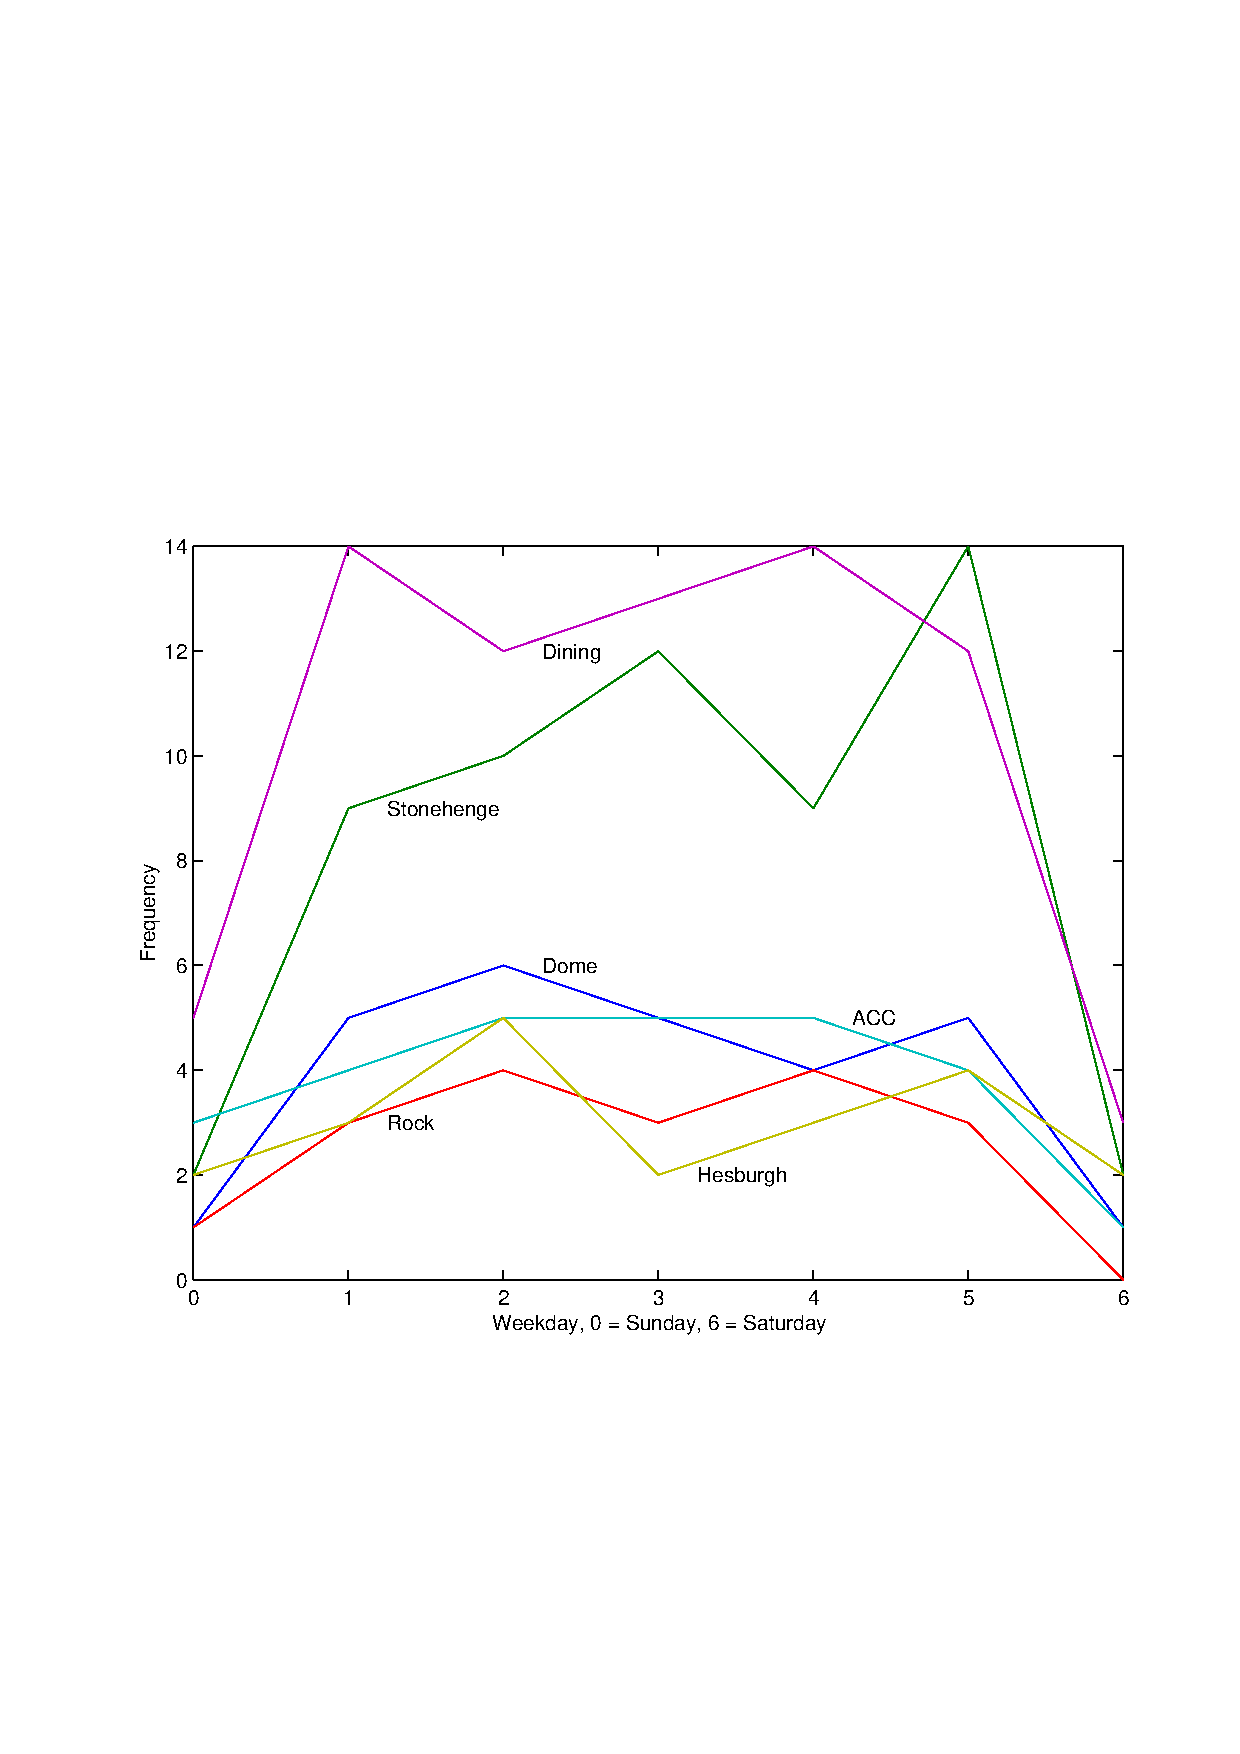
\includegraphics[scale=0.8]{sample_nd}}
    \caption{Location distributions by day of where, where the X axis
      is the weekday (0 through 6), and the Y axis is the sighting
      frequency}
    \label{fig:bogus3}
  \end{center}
\end{figure}

Gnus typically tend to come out when there are large gatherings of
humans with food.  Gnus work very hard at providing us with all the
things that we like (trees, dirt, air, etc.), and so we should freely
give them food.  They will come up and stand a respectful distance
away from you, waiting to see if they will be rewarded for their
efforts.  If you offer some food, they will take it and back off a
respectful distance in order to consume their food while leaving you
to your ``personal space.''  

\section{Groovin' Gnus}
\label{sec:groovin-gnus}

Gnus do tend to stay away from humans in their normal day-to-day
workings.  This is mainly because humans don't, for the most part,
understand what they are doing.  If a Gnu is working, and a human
approaches it, the Gnu will tend to drop whatever it is doing and run
away.  This is probably do to the tendency for humans to have ``group
meetings'' and ``productivity seminars.''  Most Gnus are deathly
afraid of such overmanagement, and run at the slightest hint of it,
for fear that it will cripple their real work.

It is interesting, however, that Gnus have chosen an Institution of
Higher Education for their BOO.\footnote{Base of Operations.}  It is
often said that:
\begin{quote}
  Academic politics are the dirtiest, meanest, ugliest, and generally
  the most low-down, in-your-face, and kick-em-while-they're-down than
  anywhere else (even Washington D.C.)  because the stakes are so low.
\end{quote}
It has been hypothesized that the Gnus are subtly trying to affect a
change for the better (i.e., eliminating the overmanagement problems)
by working the very system that they are trying to change, from
within.  That is, the graduates from Notre Dame can learn from the
examples of the Gnus here, and run screaming (or chattering) at the
slightest hint of overmanagement, and let the real work proceed
unhindered.

% % uncomment the following lines,
% if using chapter-wise bibliography
%
% \bibliographystyle{ndnatbib}
% \bibliography{example}
!
و
\verb!\chapter{فضاهای فشرده پایدار و فضاهای مرتب فشرده}
\thispagestyle{empty}
\section{فضاهای فشرده پایدار}
یک فضای توپولوژیک جزئاً مرتب (یا به طور خلاصه، فضای مرتب)، از دیدگاه آبرامسکی
\cite{abramsky2}،
مجموعه‌ای مانند $ X $ همراه 
با یک توپولوژی $ \mathcal{O} $ و یک ترتیب $ \leq $ است به طوری که گراف ترتیب در $X\times X  $ بسته باشد. بنابراین ...
\section{فضاهای مرتب فشرده}
در این  بخش به بیان ...!
را در فایل 
\LRE{\verb!tabriz-thesis.tex!}،
غیرفعال%
\RTLfootnote{
برای غیرفعال کردن یک دستور، کافی است پشت آن، یک علامت
\%
 بگذارید.
}
 کنید. زیرا در غیر این صورت، ابتدا مطالب فصل ۱ و ۲ پردازش شده (که به درد ما نمی‌خورد؛ چون ما می‌خواهیم خروجی فصل ۳ را ببینیم) و سپس مطالب فصل ۳ پردازش می‌شود و این کار باعث طولانی شدن زمان اجرا می‌شود. زیرا هر چقدر حجم فایل اجرا شده، بیشتر باشد، زمان بیشتری هم برای اجرای آن، صرف می‌شود.
\subsection{مراجع}
برای وارد کردن مراجع \پ خود، کافی است فایل 
\verb!references.tex!
را باز کرده و مراجع خود را مانند مراجع داخل آن، وارد کنید. اگر کاربر حرفه‌ای تِک هستید، پیشنهاد می‌شود که از \lr{Bib\TeX} برای 
وارد کردن مراجع استفاده کنید. نکته‌ای که باید به آن توجه کنید این است که در نسخه‌های قدیمی زی‌پرشین، 
قسمت مراجع، حاشیه‌های نامناسبی ایجاد می‌کرد. لذا در نسخه‌های جدید، این حاشیه‌ها اصلاح شده و به خاطر همین، چند دستور جدید، جایگزین شده است. بنابراین، اگه هنوز از نسخه‌های قدیمی زی‌پرشین استفاده می‌کنید، ممکن است هنگام پردازش قسمت مراجع، با خطا مواجه شوید. برای اطلاع از این دستورها، می‌توانید به تالار گفتگوی پارسی‌لاتک و یا راهنمای بسته 
\verb!bidi!
مراجعه کنید.
\subsection{واژه‌نامه فارسی به انگلیسی و برعکس}
برای وارد کردن واژه‌نامه فارسی به انگلیسی و برعکس، چنانچه کاربر مبتدی هستید، بهتر است مانند روش بکار رفته در فایل‌های 
\verb!dicfa2en!
و
\verb!dicen2fa!
عمل کنید. اما چنانچه کاربر پیشرفته هستید، بهتر است از بسته
\verb!glossaries!
استفاده کنید. راهنمای این بسته را می‌توانید به راحتی و با یک جستجوی ساده در اینترنت پیدا کنید.
\subsection{نمایه}
برای وارد کردن نمایه، باید از 
\verb!xindy!
استفاده کنید. زیرا 
\verb!MakeIndex!
با حروف «گ»، «چ»، «پ»، «ژ» و «ک» مشکل دارد و ترتیب الفبایی این حروف را رعایت نمی‌کند. همچنین، فاصله بین هر گروه از کلمات در 
\verb!MakeIndex!،
به درستی رعایت نمی‌شود که باعث زشت شدن حروف‌چینی این قسمت می‌شود. راهنمای چگونگی کار با 
\verb!xindy! 
را می‌توانید در تالار گفتگوی پارسی‌لاتک، پیدا کنید.
\section{اگر سوالی داشتم، از کی بپرسم؟}
برای پرسیدن سوال‌های خود در مورد حروف‌چینی با زی‌پرشین،  می‌توانید به
 \href{http://forum.parsilatex.com}{تالار گفتگوی پارسی‌لاتک}%
\LTRfootnote{\url{http://www.forum.parsilatex.com}}
مراجعه کنید. شما هم می‌توانید روزی به سوال‌های دیگران در این تالار، جواب بدهید.
    
در ادامه، برای فهم بیشتر مطالب، چند تعریف، قضیه و مثال آورده شده است!
\begin{definition}
مجموعه همه ارزیابی‌های  (پیوسته)  روی $(X,\tau)$، دامنه توانی احتمالی
\index{دامنه توانی احتمالی}
$ X $
نامیده می‌شود.
\end{definition}
\begin{theorem}[باناخ-آلااغلو]
\index{قضیه باناخ-آلااغلو}
اگر $ V $ یک همسایگی $ 0 $ در فضای برداری 
\index{فضای!برداری}
 توپولوژیکی $ X $ باشد و 
\begin{equation}\label{eq1}
K=\left\lbrace \Lambda \in X^{*}:|\Lambda x|\leqslant 1 ; \ \forall x\in V\right\rbrace,
\end{equation}
آنگاه $ K $،  ضعیف*-فشرده است که در آن، $ X^{*} $ دوگان
\index{فضای!دوگان}
 فضای برداری توپولوژیکی $ X $ است به ‌طوری که عناصر آن،  تابعی‌های 
خطی پیوسته
\index{تابعی خطی پیوسته}
 روی $X$ هستند.
\end{theorem}
تساوی \eqref{eq1} یکی از مهم‌ترین تساوی‌ها در آنالیز تابعی است که در ادامه، به وفور از آن استفاده می‌شود.
\begin{example}
برای هر فضای مرتب، گردایه 
$$U:=\left\lbrace U\in O: U=\uparrow U\right\rbrace $$
از مجموعه‌های بالایی باز، یک توپولوژی تعریف می‌کند که از توپولوژی اصلی، درشت‌تر  است.
\end{example}
حال تساوی 
\begin{equation}\label{eq2}
\sum_{n=1}^{+\infty} 3^{n}x+70x=\int_{1}^{n}8nx+\exp{(2nx)}
\end{equation}
را در نظر بگیرید. با مقایسه تساوی \eqref{eq2} با تساوی \eqref{eq1} می‌توان نتیجه گرفت که ...